\section{Design}
\label{sec:design}

\subsection{Design Goals}

Houdini is a security testing framework specifically designed to evaluate container isolation within Docker environments. Its primary goal is to systematically measure and evaluate a system's performance or quality against a set of predefined standards or metrics. In the context of security benchmarking for container confinement, benchmarking involves testing the effectiveness of a container's isolation mechanisms—such as namespaces, cgroups, seccomp, and other security features—by simulating real-world attack scenarios and assessing whether these mechanisms successfully prevent unauthorized access, privilege escalation, or container escapes. Essentially, it is a process of objectively comparing how well container security measures perform, identifying strengths and weaknesses, and providing a reference point for improving overall security posture. Unlike general-purpose security tools, Houdini focuses exclusively on container isolation, ensuring that tests produce reliable and reproducible results across different Docker setups. By simulating real-world attack scenarios, Houdini also verifies whether Docker’s security mechanisms successfully block actions that could lead to container escapes or privilege escalation. The framework is modular and extensible, allowing users to define new tests (tricks) to cover emerging risks, and it is built to adapt to different Docker configurations and container runtimes. Additionally, Houdini supports automation, enabling seamless integration into continuous integration (CI) pipelines for ongoing security assessments. The tool also prioritizes reproducibility by isolating tests in controlled environments, ensuring consistent results across configurations. Furthermore, it provides detailed reports that highlight the success or failure of security measures, offering actionable insights to improve container security practices.

Houdini is not only a tool for testing container isolation but also a means to optimize container privilege configurations. By systematically simulating various tasks within Docker containers, Houdini can help determine the minimal set of privileges required for a container to perform its intended function. For example, administrators can start with a container configured with broad privileges and then incrementally reduce permissions—such as Linux capabilities, seccomp filters, or resource limits, while monitoring task success. Houdini’s testing framework will identify the point at which functionality is maintained while unnecessary privileges are removed, thereby pinpointing the least privilege configuration that still allows the container to operate effectively. This approach is highly beneficial because it adheres to the principle of least privilege. Minimizing the privileges granted to a container reduces its attack surface, making it significantly harder for an attacker to exploit vulnerabilities or escalate privileges in the event of a breach. Additionally, this fine-tuning helps prevent unintended interactions between the container and the host system, leading to a more robust and secure container environment.

In order to achieve the aforementioned result, we designed \houdini with the following
goals in mind:
\begin{dgenum}
  \item \label{dg:repro}\textit{Reproducible Results.} A key goal of \houdini is to ensure that tests yield consistent and repeatable results. By controlling system variables and maintaining a structured testing environment, Houdini allows researchers and practitioners to compare results across different system configurations and security policies.

  \item \label{dg:container}\textit{Separation from the Host.} \houdini is designed to run tests inside a controlled containerized environment within a virtual machine (VM), ensuring that even if a test triggers a security vulnerability, it does not compromise the host system running the tests. This design choice enhances the safety of security evaluations, preventing unintended side effects on the underlying infrastructure.

  \item \label{dg:test}\textit{Test Case Expressiveness.} \houdini test cases (called
  \enquote{tricks}) should be maximally expressive, such that some combination of steps
  can be used to achieve and test any desired result. It should be possible to define
  a new \houdini trick and modify existing tricks without modifying the \houdini
  binary. Moreover, it should be clear from reading a defined trick precisely what steps
  are involved, the consequences of each step passing or failing, and the overall nature
  of the exploit being tested.

  \item \label{dg:failures}\textit{Focus on Observing Failures, Not Preventing Them.} Houdini is built to identify security weaknesses rather than defend against attacks.
\end{dgenum}

\subsection{Security of the Testing Environment}

If Houdini were compromised during testing, it would not necessarily pose a threat to the host system due to the design of the testing environment. Houdini is intentionally designed to operate within a controlled, containerized environment inside a VM. This means that even if a test were to exploit a vulnerability within the containerized environment, the impact would be contained within the VM, isolated from the host system and other containers. The VM itself serves as an additional layer of security, providing a buffer that prevents the compromise from reaching the host infrastructure.

\subsection{Design of Tricks}

\begin{figure}
  \label{fig:state-machine}
  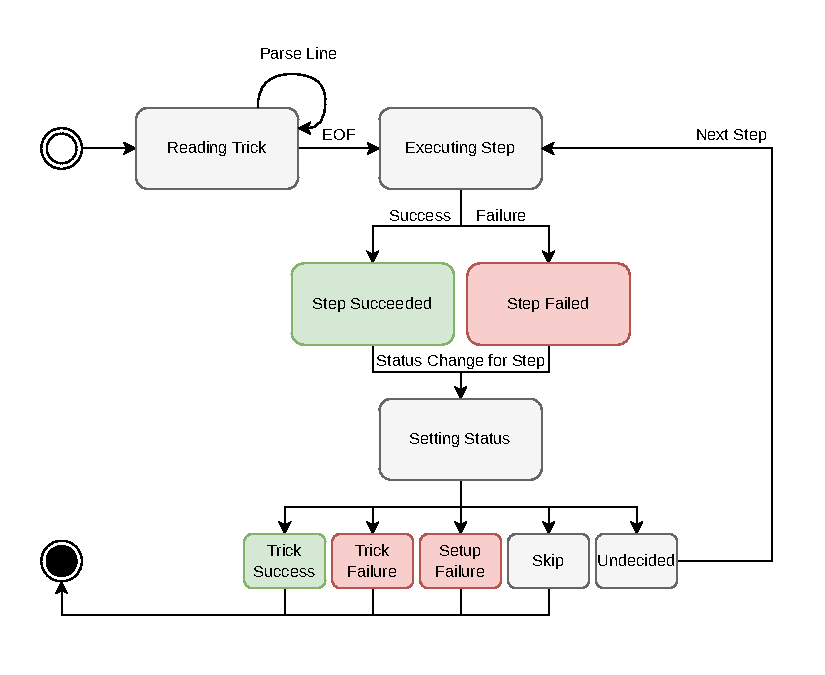
\includegraphics[width=1\linewidth]{figs/houdini-state-machine.pdf}
  \caption{A state machine diagram of Houdini running a Trick.}
\end{figure}

In containerized environments, security challenges often arise from vulnerabilities within specific components of the architecture. As such, understanding the relationships between the different components—such as container registries, images, runtime, namespaces, cgroups, and various security modules like eBPF, seccomp, and Linux capabilities—is crucial for identifying potential attack surfaces. This is where a comprehensive architecture diagram comes into play.

\begin{figure}
  \label{fig:architecture}
  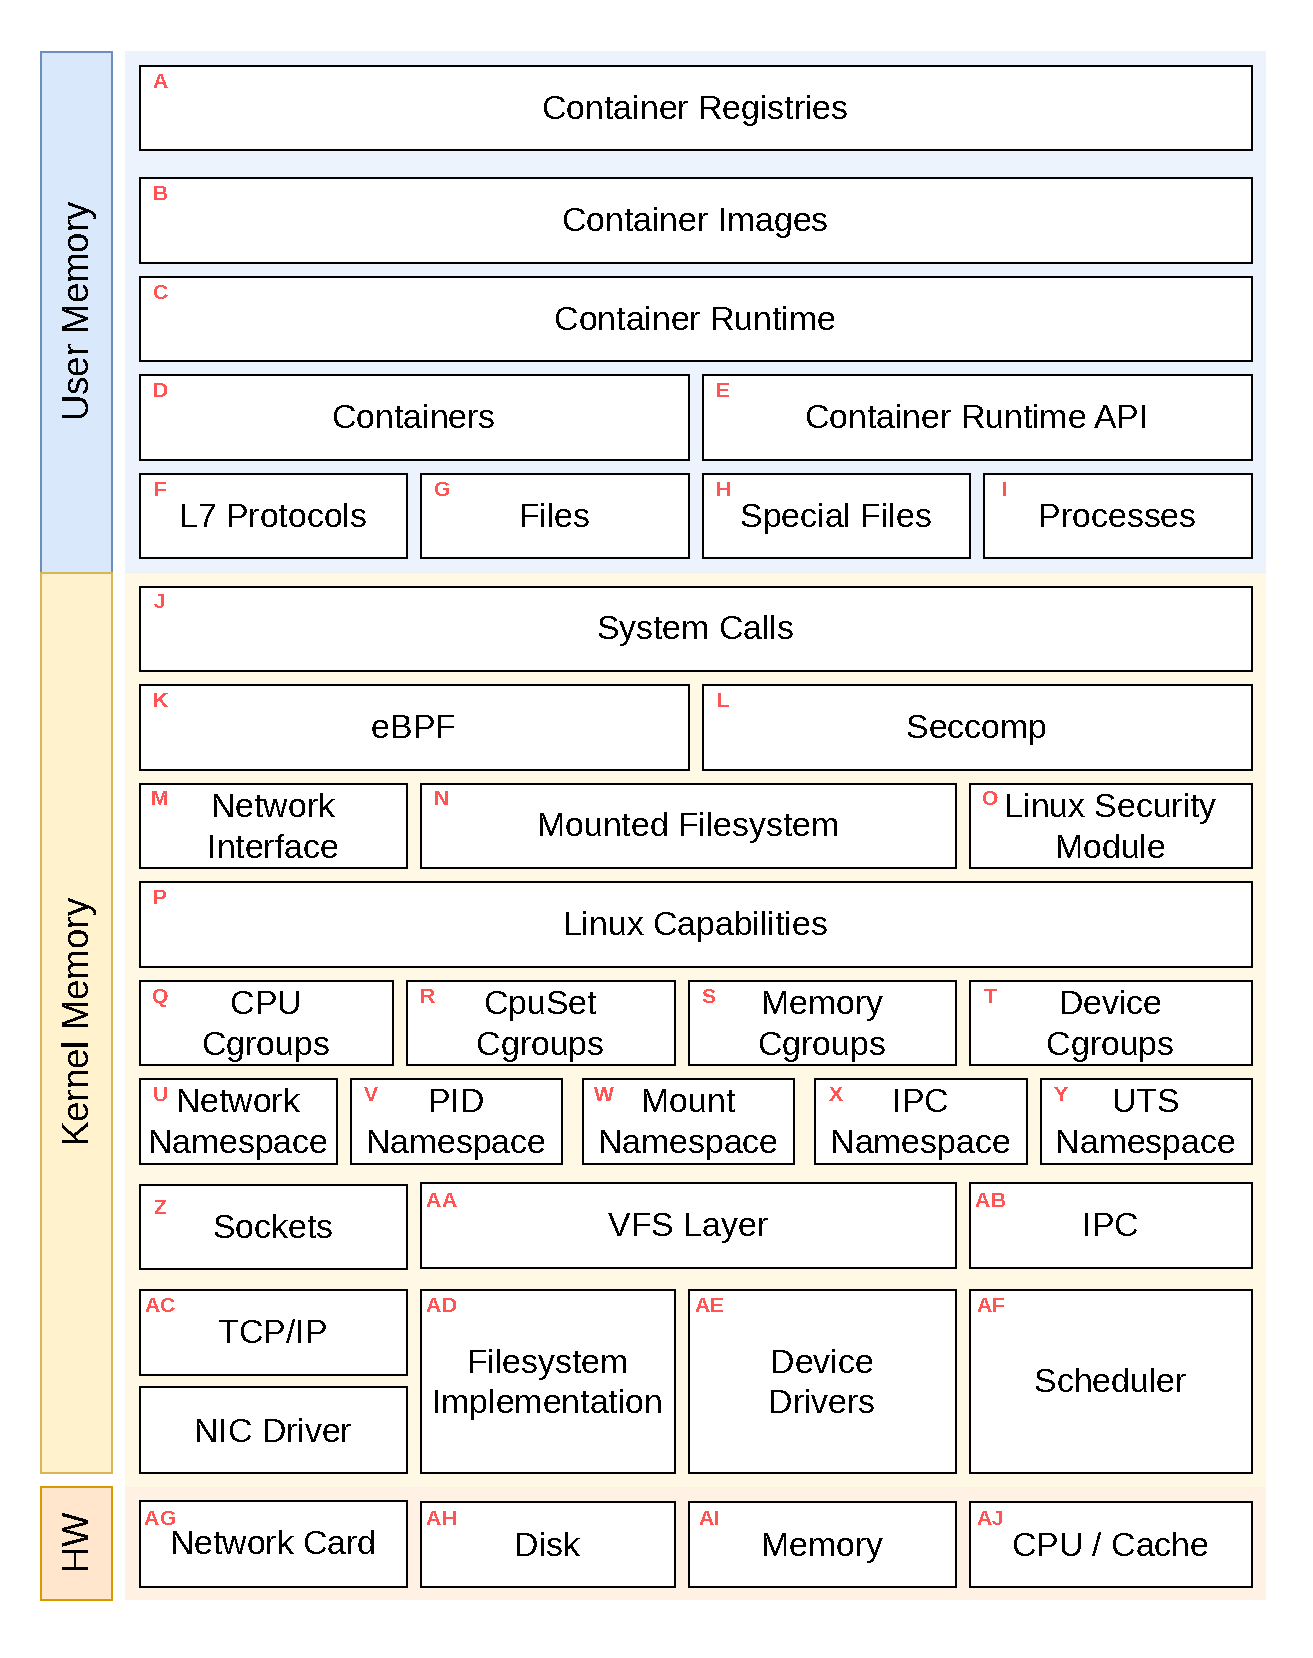
\includegraphics[width=1\linewidth]{figs/exploit-coverage.pdf}
  \caption{An architectural diagram of a container deployment environment depicting the attack surface created by its various components.}
\end{figure}

Figure 2 outlines the key components of a containerized system, highlighting the critical paths and interactions that security tests should focus on. Security testing should aim to cover these components extensively to ensure that vulnerabilities in any of these layers are adequately addressed. However, some components, like network interfaces, system calls, and cgroups, are more frequently targeted in real-world attacks and thus warrant more attention in testing. The diagram will guide our understanding of which components to prioritize during testing, ensuring that our coverage is both thorough and effective.
